\problem{Initial Value Problem}


\solution

\part 


The following matlab code is used to solve exercise 1:

\begin{verbatim}
function LAB04ex1
t0 = 0; tf = 40; y0 = [10;60];
[t,Y] = ode45(@dYdt,[t0,tf],y0) %,[])%,a,b,c,d);
y = Y(:,1); v = Y(:,2);
figure(1);
plot(t, y, 'b-+'); ylabel('y'); legend('y(t)');
hold on
plot(t, v, 'ro-'); ylabel('v'); legend('v(t) = y''(t)');
hold off
xlabel('t');
ylim([-1.5, 1.5]);
grid on;
figure(2);
plot(y, v); axis square; xlabel('y'); ylabel('v'); % plot the phase plot
ylim([-1.5, 1.5]);
xlim([-1, 1]);
grid on;

function dYdt = f(t, Y) % f(t,Y,a,b,c,d)
y = Y(1); v = Y(2)
dYdt = [v; cos(t) - 4*v - 3*y];
\end{verbatim}

The code simply integrates the equation and plots the resulting functions and their phase diagram. 
This shows two oscillating functions offset from one another, and a stable equilibrium which is reached after a certain amount of time. A legend and grid lines are shown. Each figure is intentionally given a full page so that detail can be shown.

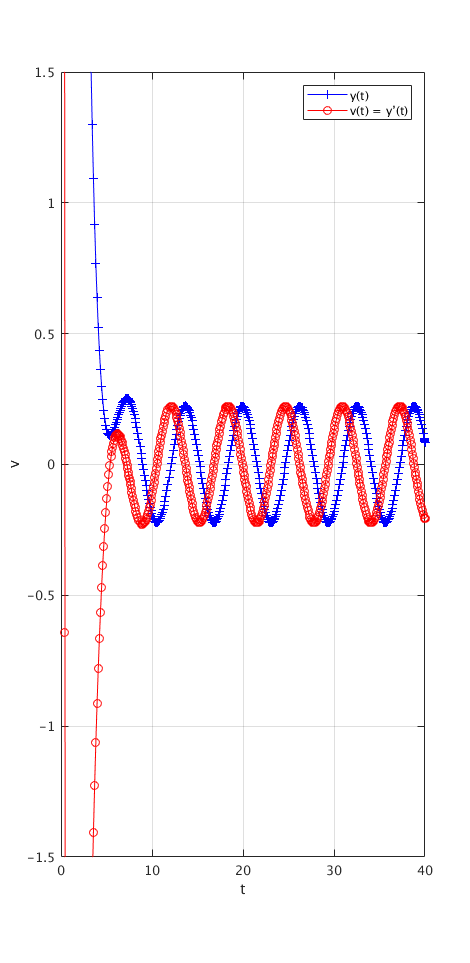
\includegraphics{00} \\
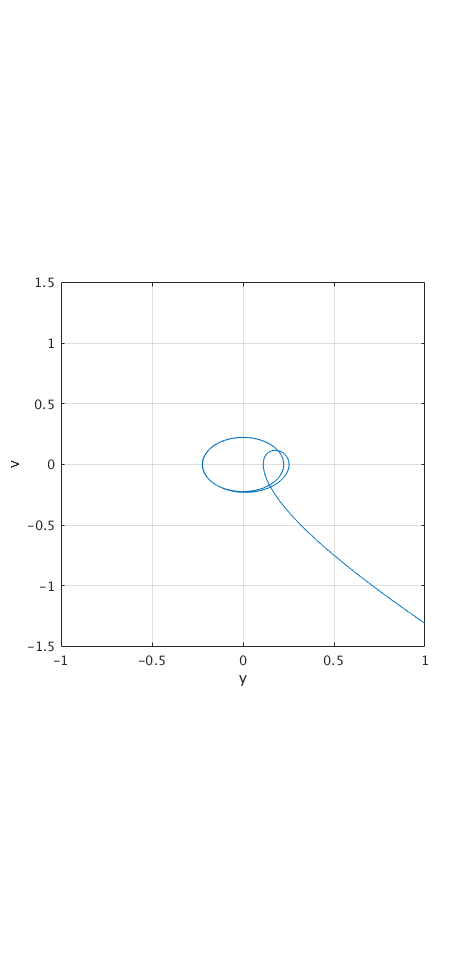
\includegraphics{01}


\part

Approximately, the value of $t = 0$ makes $y$ maximum, based on my graph and data. This is because $y$ starts at sixty when $t$ is $0$, and then decreases from there until $y$ reaches an oscillating section, which is discussed in the next part.

\part
 
After an initial period, the equation for $y$ appears to be oscillating between two values, which would make it \emph{stable}. 

\part

When the initial starting location is changed to $(1.5, 5)$, the long-term stability of $y$ is not affected. 
Despite the fact that the path starts in a new location, it is attracted into the same ``orbit''. 
This can also be seen in the phase diagram (next pages).
However, this does affect the local maximum value of $y$, as it begins lower.

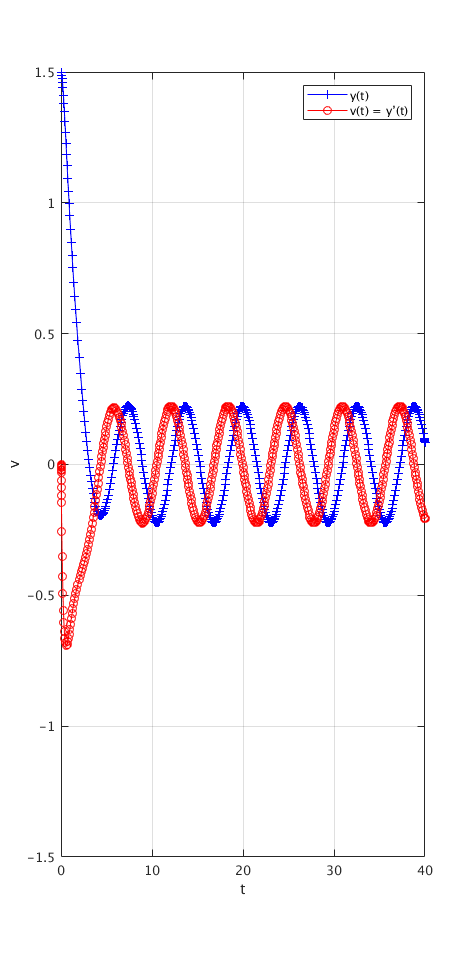
\includegraphics{11} \\
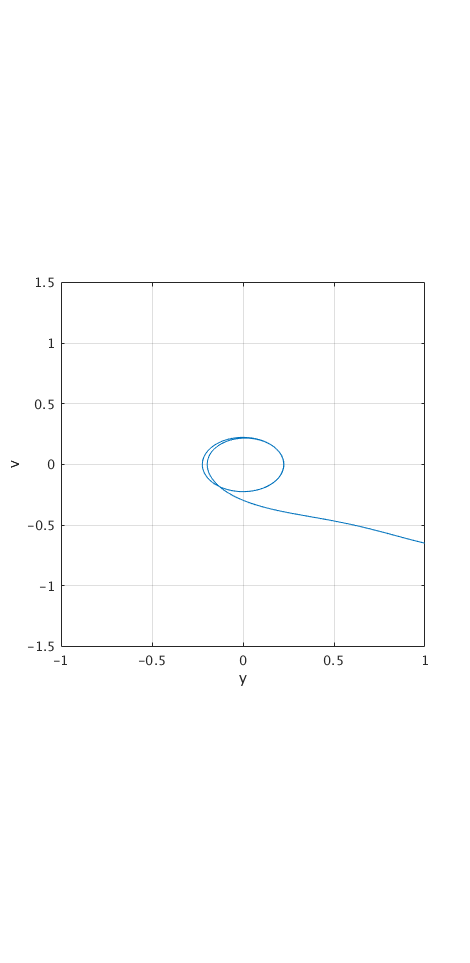
\includegraphics{12}

